\onehalfspacing 
\label{chapter2}
\section{Variety and Repetition}
In response to Kyle Adams' seminal \textit{Music Theory Online} article ``Aspects of the Music/Text
Relationship in Rap,'' Justin Williams remarks on a significant phenomenological development in rap 
music production, following the genre's move from the turntable, to the studio, and even more recently
to the Digital Audio Workstation (DAW). He writes:
    \begin{quote}
        \small ``In terms of rap music recordings, the idea of a completely fixed loop is largely fictitious.
        There may be a set of layers which we could term the `basic beat' which repeats intact for certain
        durations of time, but one would be hard-pressed to find an entire musical complement that stays the 
        same throughout. Rap music’s layers will more often than not fluctuate throughout a given song, with
        sonic additions and subtractions, manipulations of digital samples, and even sharp changes in aspects 
        of the basic beat.''\footnote{\cite{justinawilliamsBeatsFlowsResponse2009}. It is worth noting that 
        Adams does not necessarily dispute the occurrence of development within an accompaniment as a phenomenon,
        but he does maintain that the unchanging elements of the beat function as ``primary accompanimental
        layers'' (See \cite{kyleadamsPeopleInstinctiveAssumptions2009}.)}
    \end{quote}
Repetition and variation are equally essential within the musical lexicon of the rap instrumental. Adams 
notes that even as the locus of rap music-making moved into the studio, producers remained adherent to 
the break-beat based origins of the genre, and so structural elements of the hip-hop beat tend to repeat
within a four to eight bar, often simple quadruple metrical space. At the same time, Williams' observations
point towards a preference for variation within repetition, made feasible by newer technologies for sampling,
manipulating, and composing with pre-recorded digital materials.

Whether the hip-hop beat is primarily repetitive or primarily developmental is indeterminate because 
both variables exert influence over the creative process; it is more valuable to interrogate how different
producers use these phenomena to aesthetic or rhetorical ends. To invoke Loren Kajikawa's notion of
sounding, variety and repetition factor into how ``rap artists produce (and listeners interpret) musical
meanings at the level of the song.''\footnote{\cite{lorenkajikawaSoundingRaceRap2015}, 2.} Although Kajikawa
focuses on the sounding of racial and gender identities, his critical apparatus may also extend to producers'
use of music to identify with or against their perception of a hip-hop mainstream. I therefore argue that
underground producers make beats that code themes and identities in conversation with the hip-hop mainstream
while rappers simultaneously declare allegiance to the underground within their flow. Because, as Kajikawa
notes,``rap has cultivated a mainstream audience\textellipsis by promoting highly visible (and often
controversial) representations of black masculine identity,''
\footnote{\cite{lorenkajikawaSoundingRaceRap2015}, 5.} the hip-hop underground operates as a 
space to subversively play with these representations.

As with any sub-generic distinction predicated on narratives of authenticity, I use the term
\emph{underground} trepidatiously, knowing full well it has as many meanings as it has users. What I 
call the underground signifies a space where deviation from the mainstream is acceptable, perhaps even
preferable. This is not a value judgement, nor an all-encompassing definition of either mainstream or
underground. My definition is necessarily vague because these are elusive terms, yet they hold importance
because they represent \textit{de facto} ``imagined communities'' with which rappers, producers, and
listeners identify.\footnote{Many scholars, including Williams and Joseph G. Schloss, have theorized 
hip-hop culture as an imagined community, borrowing the term from Benedict Anderson's writings on national
identities. Anderson uses the term to refer to communities in which ``[many] will never know most of their
fellow members, meet them, or even hear of them, yet in the minds of each lives the image of their
communion'' (see \cite{benedictandersonImaginedCommunitiesReflections2006}, 6).

In hip-hop studies, scholars argue that the imagined community grants cohesion to the discursive 
nature of hip-hop. Both Schloss and Williams use it to describe overlapping spheres of association,
influence, and reference that exist within the hip-hop art world. Through the medium of a sound object
(verse, song, album, beat, etc.), a member of the imagined community en- or de-codes the traditions,
histories, and identities of the whole (see \cite{josephgschlossMakingBeatsArt2004}, 4, and
\cite{justinawilliamsRhyminStealinMusical2013}, 12-13.)}

In this chapter, I argue that producers work with rappers to sound the hip-hop underground by using
variety within their construction of the beat, articulating alternative identity; I base this argument 
in transcriptions that illustrate developmental and repeating elements within the musical texture. My case
studies show that underground producers tend to deviate from expectations concerning form. Highlighting
sample-based and live-tracked approaches to beat-making, I trace methods of sample and loop manipulation 
such as \emph{resampling (or recomposing)}, \emph{choking}, \emph{slipping}, \emph{glitching} as producers'
means of variation. Lastly, I contend that underground hip-hop is sounded by an overarching aesthetic of
diversity, linking the sound of the underground to Olly Wilson's heterogeneous sound ideal of
African-American music.\footnote{\cite{ollywilsonHeterogeneousSoundIdeal1992}.}

%\clearpage
\section{Methods of Transcription and Analysis} \label{methodsoftranscription}
I use transcription in this chapter\textemdash indeed, overall in this project\textemdash despite 
knowing that it introduces a level of abstraction from both the musical practice and perceptual experience 
of my hip-hop repertory. Scholars such as Joseph G. Schloss have meaningfully analyzed hip-hop production
while eschewing transcription altogether on ethical and aesthetic
grounds.\footnote{\cite{josephgschlossMakingBeatsArt2004}, 13-15.} Others, like Kajikawa and Adam 
Krims, have employed methods of transcription that move away from standard notation in the Western 
Classical tradition.\footnote{\textit{Cf.} \cite{lorenkajikawaSoundingRaceRap2015}, 29-30 and 36-37;
\cite{adamkrimsRapMusicPoetics2000}: 105-110.} Still others, including Adams and Robert Komaniecki, 
rely primarily on standard notation in order to present their arguments within traditional spheres of
music-theoretical discourse.\footnote{\textit{Cf. }\cite{kyleadamsMetricalTechniquesFlow2009};
\cite{robertkomanieckiAnalyzingCollaborativeFlow2017}.} Each approach holds its own merit, and 
each privileges a different audience: the creator, the listener, and the academic.

Although I understand Schloss and others' reticence to transcribe rap music, my choice to do so
grows out of the mode of deep listening requisite to creating a transcription. By using transcription,
I do not aim to apply ``the tools of notation and analysis developed for the study of Western Classical
music\textellipsis uncritically to rap music.''\footnote{\cite{lorenkajikawaSoundingRaceRap2015}, 12.}.
Instead, I offer them as a subjective realization of my ``living inside'' the musical object for a
time.\footnote{\cite{peterwinklerWritingGhostNotes1997}: 200.} Transcription therefore offers the best 
method of communicating my experience within a written medium.

I use both standard and non-standard styles of transcription in this chapter to distinct ends. 
First, I use tables that I call ``roadmaps'' to provide an overview of musical form, noting the 
relationship between sections, samples, and durations.\footnote{Each roadmap in the chapter has a
corresponding expanded version that details the function and relationship of each instrumental layer 
and counting durations by samples. These expanded versions can be found in the appendix beginning on
p.~\pageref{appendix:fullroadmaps}.} I also pay special attention to when producers create variety 
within the musical texture using one of the four methods listed above and defined below. In addition, 
I use standard notation to create a musical ``snapshot'' of the beat at distinct points in the musical
texture. These snapshots allow me to discuss the function of particular musical layers and also to more
closely analyze the methods of creating variety outlined in the roadmaps. Using staff notation requires 
a certain reduction of the rhythmic and textural complexity of my pieces, but I use these snapshots 
in an effort to draw out the moments that cannot be easily notated within them.

As my roadmaps show, underground producers play with expectations for form in mainstream hip-hop, 
typically avoiding the \emph{verse-hook} formal model. Ben Duinker defines verse-hook form in hip-hop 
as an analog to \emph{verse-chorus} form in popular music, and he shows that hip-hop's assimilation to
mainstream popular culture has correlated with the increase of this
form.\footnote{\cite{benduinkerSongFormMainstreaming2020}, 105.\label{duinkerhookdef}} At the same time, 
he differentiates verse-hook from verse-chorus on account of the means by which hooks fulfill the role of
refrains.\footnote{Duinker notes that, unlike choruses, hooks do not lend themselves to ordered 
pairings that David Temperley labels ``verse-chorus units'' or VCUs, nor do hooks use the same features
of differentiation that Temperley notes in rock songs. See \cite{davidtemperleyMusicalLanguageRock2018},
159\textit{ff}.} Nevertheless, the correlation between verse-hook form and the mainstreaming of rap music
in popular culture offers underground producers a model of song form with which to converse in their 
effort to create hip-hop in dialogue with expectations.

The producers in my repertory tend to make beats using the section types Duinker identifies\textemdash
hooks, instrumentals, and ``looser-organized'' sections.\footnote{\cite{benduinkerSongFormMainstreaming2020},
95-101.} Admittedly, defining the function of a section based solely on production is somewhat subjective,
especially because underground emcees through-compose their texts. How a producer chooses to order musical
material, then, can either clarify or contrast the form projected by the vocal performance. I believe
underground producers use form playfully in relation to the rapped text.

My snapshots show how underground producers treat variety within formal sections as aesthetically
preferential to unaltered loops and samples. Duinker notes that within verses particularly, the 
looped sequence of the beat can change gradually through the introduction or subtraction of loops 
that are generally one, two, or four measures in length via \emph{layering}.
\footnote{\cite{benduinkerSongFormMainstreaming2020}, 96.} While underground producers occasionally
use layering, they also use techniques that create drastic changes, even within a formal section. 

Specifically, underground producers introduce changes within the beat using techniques that mimic
the live, improvisatory roots of hip-hop; these are the methods of alteration I introduced above. 
In order to present my close readings of each case study below, I will define \emph{resampling (or
recomposing)}, \emph{choking}, \emph{slipping}, \emph{glitching} in the paragraphs that follow.

I use the term resampling to encapsulate any changes a producer makes to a sample while still presenting
it as a complete loop. The term reflects a function offered to producers who use samplers like the Roland 
SP series or DAWs like Ableton, where any audio can be played with post-processing effects and other
manipulations while being captured on a new sample pad or audio track. This allows producers to make 
changes to the pitch of a sample, the rhythmic sequence of components within a sample, and the engagement
of effects in real time and thus becomes a method for altering pre-recorded material. Recomposing 
functions much like resampling but particularly for producers who record live or software instruments
alongside samples. A recomposition occurs when a producer takes a repeated loop and alters its content,
either with new pitch and rhythmic material or by changing some element of the loop's timbre. 

Sample choking deals with muting a portion of the loop or sample completely, cutting it off as a 
sound source. Compared to removing a layer (which occurs gradually), sample choking happens within 
the length of a single sample or loop. Sample chokes can occur at lengths perceptually experienced 
as a beat, as well as in short and/or rapid rhythmic values below the point of meaningful notation. 
Like resampling or recomposing, choking plays with the perception of repetition within the loop but 
does not completely disrupt it.

In comparison, glitching and slipping challenge a listener's sense of the repetitive structure 
more drastically and clearly mark a change to repeating sonic objects in the mix. Glitching takes 
a portion of a sample or loop and ``chops'' it, then repeats the selected portion, often stretching 
portions of audio shorter than a beat to take up space longer than a beat. Glitching interrupts the 
musical texture in a way comparable to scratching a vinyl record would in turntabling.\label{glitch} 
Slipping, by contrast, disturbs repetition more subtly. When two samples of slightly varied lengths 
loop over long periods of time, they slip apart, widening the gaps between them. Alternatively, 
producers slip samples through re-triggering onsets rather than looping them, adding micro-rhythmic 
delay. Both methods create a disalignment of sample and loop onsets.

As my analyses below demonstrate, underground producers use these compositional techniques to create 
variety within the sonic profile of their beats. In both sample-based and live-tracked approaches to
beatmaking, underground producers create internal and formal variety in dialogue with the emcee's vocal
delivery. Their alterations to samples, loops, and form introduce heterogeneity to the musical work and
articulate an underground aesthetic in comparison to mainstream approaches.

%\clearpage
\section{Sample-Based Case Studies} \label{samplebased}
The contemporary practice of sample-based beatmaking links back to hip-hop's origins, echoing the 
practice of looping breakbeats on the instrumental b-sides of vinyl records pioneered by DJs like 
Kool Herc and Grandmaster Flash.\footnote{\cite{triciaroseBlackNoiseRap1994}, 51.} Because producers 
who sample do not need to be multi-instrumentalists to create a full musical texture, sample-based 
beatmaking democratizes music production; but furthermore, it imbues hip-hop with a sonic lineage and
particular type of nostalgia. Tricia Rose likens the ingenuity of hip-hop production to other forms of 
Black creativity, where making something good often involves ``making\textellipsis out of the
scraps\textemdash creating a delicacy of the undesirable, discarded parts.''
\footnote{\cite{triciaroseHipHopWarsWhat2008}, 264.} In the underground, the process of 
selecting a sample, re-contextualizing it in a new space, and exploring the full extent of variety 
it may hold seems to be a look backwards to this tradition and, thus, a way of honoring a broader 
history of the ingenuity of Black Americans.

\phantomsection
\subsection*{\centering MF DOOM's ``One Beer''}  
\addcontentsline{toc}{subsection}{MF DOOM's ``One Beer''}

    \begin{table}[ht]
        \centering
            \begin{tabular}{|c|c|c|c|l|}
                 \hline
                  Section         & Timecode & Duration & Sample              & Note                    \\ \hline
                  Intro           & 0:00     & 8 Bars   & ``Huit Octobre'' I  & Choked in Bar 8         \\ \hline
                  Verse 1A        & 0:20     & 16 Bars  & ``Huit Octobre'' II &                         \\ \hline
                  Verse 1B        & 1:02     & 16 Bars  & ``Huit Octobre'' II & Choked in Bar 0.4       \\ \hline
                  \sout{Hook}     & 1:43     & 8 Bars   & ``Huit Octobre'' I  & Choked in Bar 8.3-4     \\ \hline
                  Verse 2B        & 2:03     & 8 Bars   & ``Huit Octobre'' II & Choked in Bar 0.4, 8.4  \\ \hline
                  \sout{Verse 2C} & 2:24     & 16 Bars  & ``Huit Octobre'' II & Choked in Bar 0.4       \\ \hline
                  Skit            & 3:06     & 26 Bars  & \textit{Spider-Man} & Resampling, drum improv \\ \hline
             \end{tabular}
        \caption{Condensed Roadmap to MF DOOM and Madlib's ``One Beer.''}
        \label{tab:onebeer}
    \end{table}

Madlib produces ``One Beer'' using two samples from the French funk band Cortex's ``Huit Octobre 1971.''
Outlined in Table~\ref{tab:onebeer}, Madlib sequences these two samples with a somewhat normative approach
to form, in contrast to DOOM's through-composed verse. Madlib starts ``One Beer'' with an eight-bar
introduction built from the first sample, followed by two sixteen-bar verse-parts built from the second.
He then switches back to the first sample, making space for a hook, but DOOM's verse continues over this
projected boundary. After eight bars, the second sample re-enters for another twenty-four, creating a 
nearly parallel second verse area for DOOM. Madlib and DOOM project contrasting forms in their respective
roles as producer and rapper, and the dissonance between the two creates heterogeneity between the text 
and the instrumental.

Madlib also introduces heterogeneity within the beat itself, primarily through musical disparity in 
the selection of sampled portions from ``Huit Octobre.'' His first selection, 1:58-2:09 of Cortex's
recording, is pitched up slightly sharper than a whole step, tonicizing F-sharp. Shown in
Figure~\ref{fig:onebeerintro}, the sample grooves in a triplet eighth swing, featuring synth and bass 
in octaves arpeggiating I$^{b7}$ and a skeletal drum part emphasizing backbeats. When the track returns 
to the first sample, the relative stasis of the musical elements grants the sample a hook-like function.

    \begin{figure}[ht]
        \centering
        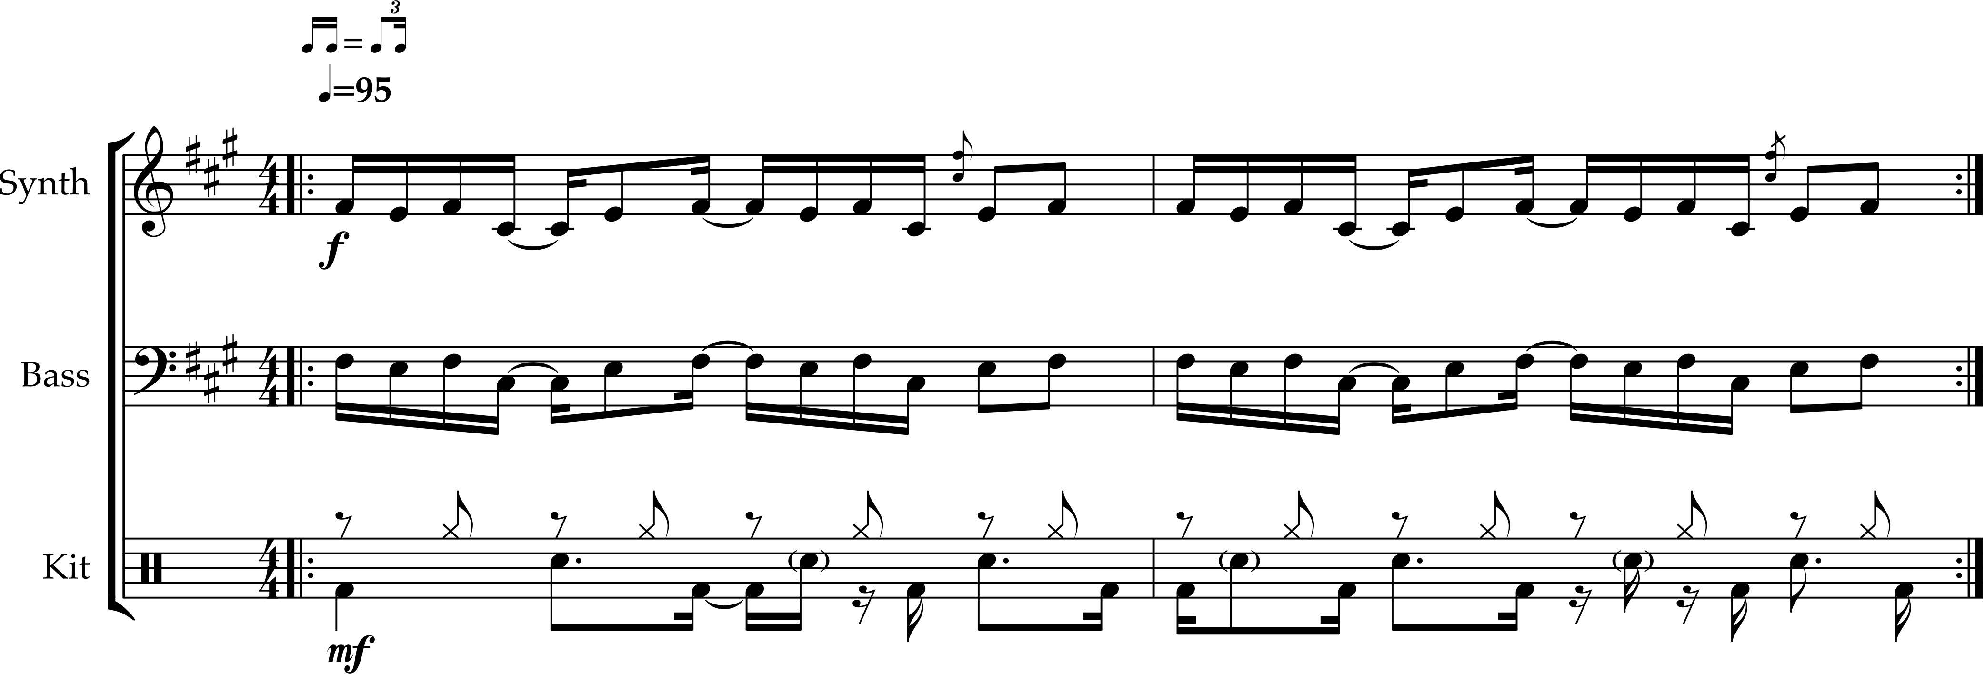
\includegraphics[width=\textwidth]{images/figures/chp 02/000019onebeerintro.pdf}
        \caption{Snapshot of Madlib's first sample in ``One Beer,'' 0:00-0:19.}
        \label{fig:onebeerintro}
    \end{figure}

The first sample sounds like a hook for two reasons. First, it is texturally distinct from the sample 
which underscores the verse portion of ``Huit Octobre,'' the primary instrumental criterion Duinker
identifies for distinguishing hooks from verses.\footnote{\cite{benduinkerSongFormMainstreaming2020}, 99.}
Second, it is created from a shorter, more singularly-focused musical idea. Its harmony, which Adams 
typifies as \emph{repetitive}, is created from two arpeggiations of a one-measure idea in rhythmic unison,
only with slightly varied articulations in each statement.
\footnote{\cite{kyleadamsHarmonicSyntacticMotivic2020}. The three categories Adams provides for 
harmony in hip-hop are repetitive, oscillating, and expansional, all of which I touch on throughout
the course of this chapter.} Overall, this section is sparser in texture and musical material, and 
Madlib uses this contrast as a point of arrival.

Madlib contrasts the first sample with his selection of the second, 0:23-0:25 of the Cortex recording.
Although also pitched up slightly sharper than a whole step, this portion slows to 92 bpm from 95 bpm 
and has a straight rhythmic feel. As Figure~\ref{fig:onebeermain} shows, both the overall musical texture
and harmonic content of this sampled section have thickened in comparison to the first. Playing distinct 
and more typical instrumental roles, the bass and synth underscore a vocal part, and the three create new
oscillating harmonies.

    \begin{figure}[ht]
        \centering
        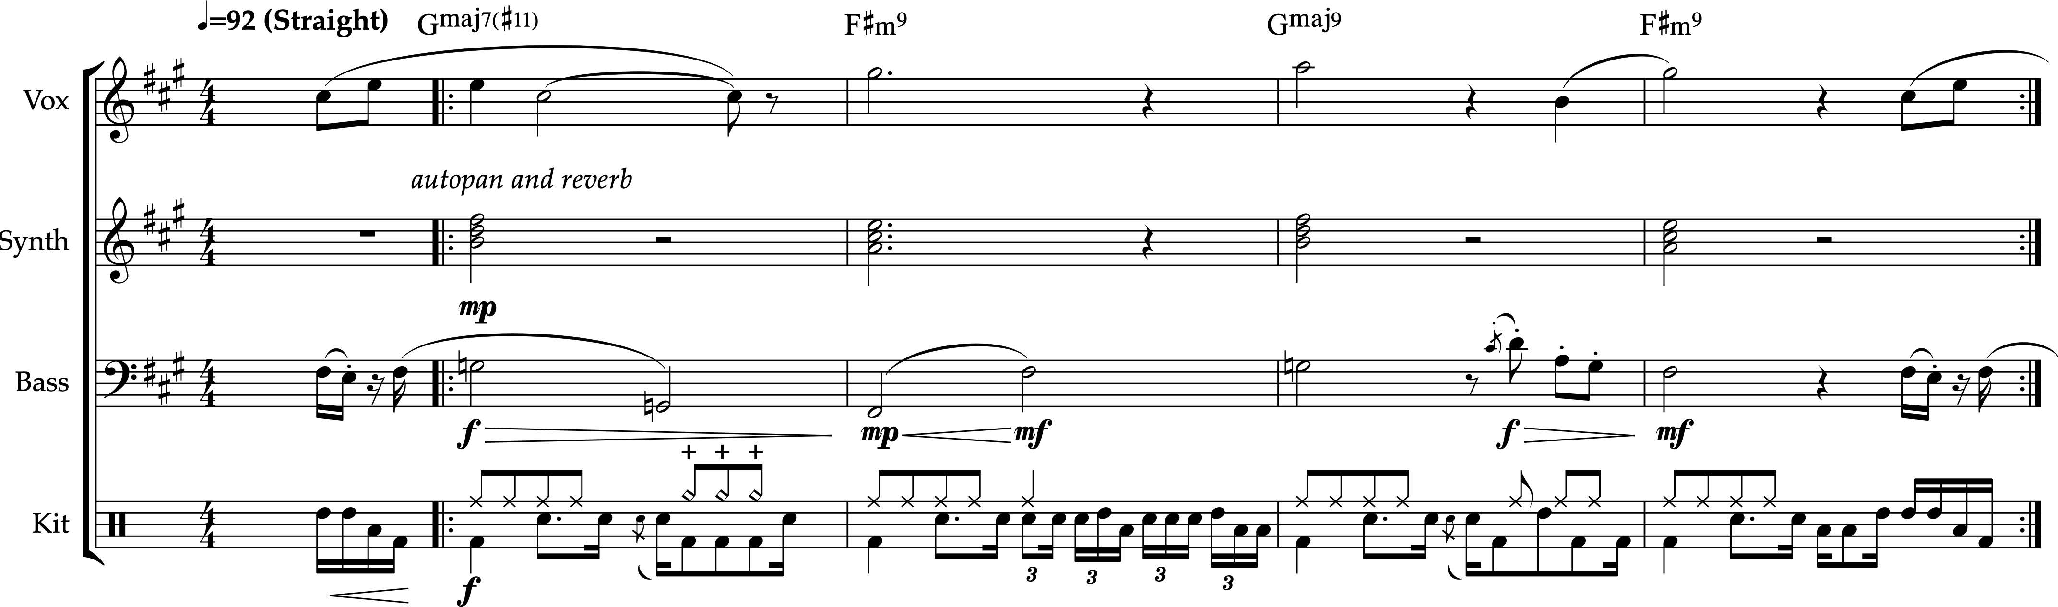
\includegraphics[width=\textwidth]{images/figures/chp 02/020031onebeermain.pdf}
        \caption{Snapshot of Madlib's second sample in ``One Beer,'' 0:20-0:31.}
        \label{fig:onebeermain}
    \end{figure}

Perhaps the most prominent shift in texture comes with the rhythmic complexity of the drum part in the 
second sample. Like the fuller harmony, the drums fill up sonic space using distinctive fills and 
striking timbres throughout the four bar loop; this culminates in the prominence of the two-beat long 
triplet eighth fill in m. 2 of Figure~\ref{fig:onebeermain}. As Schloss notes, producers often choose 
their samples based on the aesthetic delight they experience concerning timbre, especially seeking drum
sounds.\footnote{\cite{josephgschlossMakingBeatsArt2004}, 141-142.} Certainly, this second section 
luxuriates in the sonic quality of the drums.

Comparing the texture, harmony, and groove of each of Madlib's samples illustrates how internally 
varied ``One Beer'' is. Although Madlib makes use of some of the methods of altering samples\textemdash
particularly, choking the sample to delineate sectional transitions\textemdash his primary method of
introducing variety in the main part of ``One Beer'' is through the juxtaposition of the two lead samples.
Juxtaposing musical elements in this manner aligns with Wilson's heterogeneous sound-ideal, particularly
because of the resulting rhythmic clash and  timbral stratification across sample
boundaries.\footnote{\cite{ollywilsonHeterogeneousSoundIdeal1992}, 328-329.}

The final skit section of ``One Beer'' functions as a culmination of Madlib's stylistic juxtapositions. 
The skit's music is built from a looped portion of the soundtrack to ``Dr. Doom, Master of the World,'' 
an episode of the 1981 animated \textit{Spider-Man} television series. He combines dialogue from this 
episode with another selection from ``The Fantastic Four Meet Dr. Doom,'' a 1978 episode of \textit{The 
New Fantastic Four}. Beneath this, Madlib improvises a through-composed drum sequence articulating the
boom-bap structure of kick and snare common in hip-hop. All in one track, Madlib draws on a ``rich 
assortment of multimedia borrowings, references, and parodies that operate in hip-hop music as a
whole.''\footnote{\cite{joannademersSampling1970sHipHop2003}: 42.} This juxtaposition is his method 
of sounding DOOM's particular brand of alternative identity.

\phantomsection
\subsection*{\centering Kendrick Lamar's ``Rigamortus''}
\addcontentsline{toc}{subsection}{Kendrick Lamar's ``Rigamortus''}

    \begin{table}[ht]
        \centering
            \begin{tabular}{|c|c|c|c|l|}
                \hline
                Section  & Timecode & Duration & Sample        & Note \\ \hline
                Intro    & 0:00     & 4 bars   & ``The Thorn'' & \\ \hline
                Hook     & 0:10     & 6 bars   & ``The Thorn'' & Full sample plays \\ \hline
                Verse 1A & 0:27     & 12 bars  & ``The Thorn'' & \\ \hline
                Verse 1B & 0:59     & 10 bars  & ``The Thorn'' & Improvisatory sample choking \\ \hline
                Hook     & 1:26     & 6 bars   & ``The Thorn'' & Lead sample slips backwards \\ \hline
                Verse 2A & 1:43     & 6 bars   & ``The Thorn'' & \\ \hline
                Verse 2B & 2:04     & 8 bars   & ``The Thorn'' & Alternating sample choking \\ \hline
                Hook     & 2:31     & 6 bars   & ``The Thorn'' & Improvisatory sample choking\\ \hline
            \end{tabular}
        \caption{Condensed roadmap to Kendrick Lamar and Willie B's ``Rigamortus.''}
        \label{tab:rigamortus}
    \end{table}

The production team for ``Rigamortus''\textemdash Willie B and Sounwave\textemdash use Willie Jones 
III's up-tempo jazz track ``The Thorn'' as the lead sample,  singling out 0:13-0:20. In ``The Thorn,'' 
the combo groups simple quadruple meter into 3+3+2 beat divisions to underscore a saxophone and 
trombone theme that ends with a pickup figure. This texture is detailed in Figure~\ref{fig:thethornfull},
which highlights the pickup boxed in red.

    \begin{figure}[ht]
        \centering
        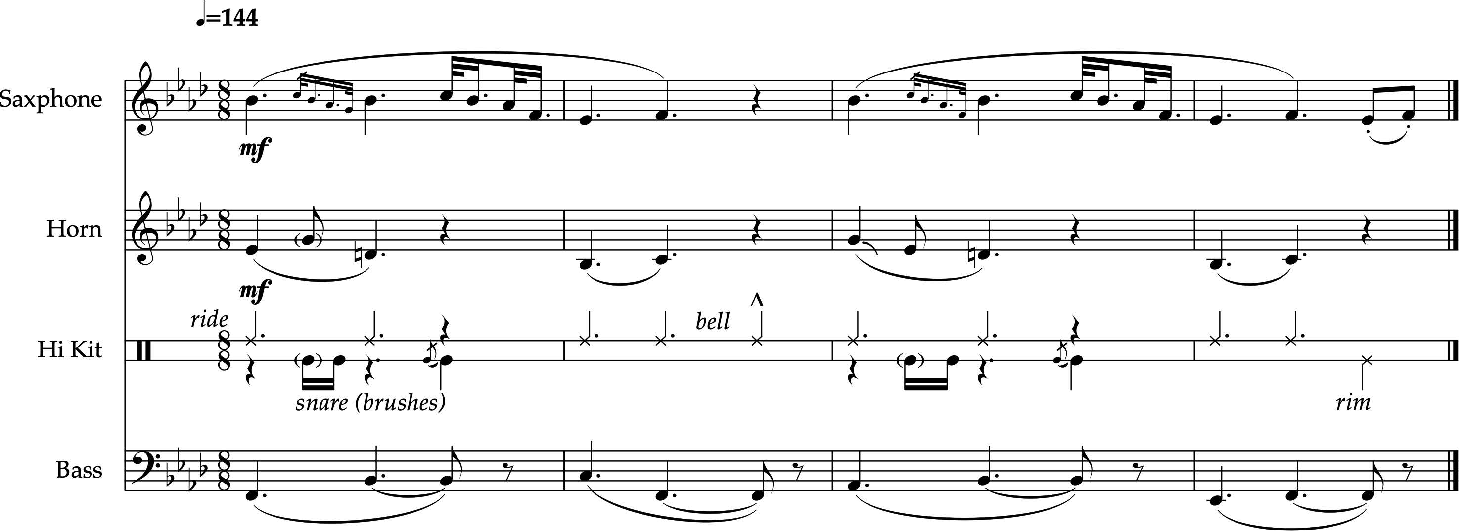
\includegraphics[width=\textwidth]{images/figures/chp 02/013020thethornfull.pdf}
        \caption{Snapshot of the sampled portion of ``The Thorn,'' 0:13-0:20.}
        \label{fig:thethornfull}
    \end{figure}

``Rigamortus'' begins with a nearly unadulterated triggering of the first two measures of the sample.
The only changes the producers make are filtering out the low end and pitching the sample up slightly 
sharper than four semitones. In its new context, the two-bar phrase sounds as a one-bar unit within a 
down tempo hip-hop context. This is confirmed when, as shown in Table~\ref{tab:rigamortus}, the full
four-measure sample is presented beneath Lamar's hook as a two-bar unit. Within the first verse, Willie B
and Sounwave also layer in a drum sequence and sub bass drone on a low A using a filter sweep to demarcate
their entrances. Figure~\ref{fig:rigamortusnoslip} shows the relationship of the sample (now in rhythmic
diminution) to the other elements of the musical texture; this structure repeats unchanged from 0:43-0:55,
with only slight choking of the lead sample.

These new musical elements recontextualize ``The Thorn'' within repetitive harmony that primarily 
sounds an A minor tonic function within a simple quadruple groove. The sample, drum, and bass each 
help ground the listener within Lamar's complex vocal delivery and the complicated approach he uses 
to form with his text. Specifically, Lamar's vocals complicate form with shifts in text and delivery. 
In Verse 2, Lamar briefly recapitulates the ``He Dead!'' call-and-response text from the hook, bisecting
the verse. He also restates the hook text at the beginning of Verse 2A, repeating ``Got me breathin' 
with dragons'' to set up a new rhyme structure and flow in the second verse. At the close of the Verse
2B, Lamar modulates into a higher and more rhythmically intense register, one that he identifies with 
his ``Gemini'' alter-ego.\footnote{\cite{chrismenchTrackingManyVoices2017}.} The producers thus create
contrast through simplicity, using discrete, simplistic musical elements for the track's entirety.

\begin{figure}[ht]
    \centering
    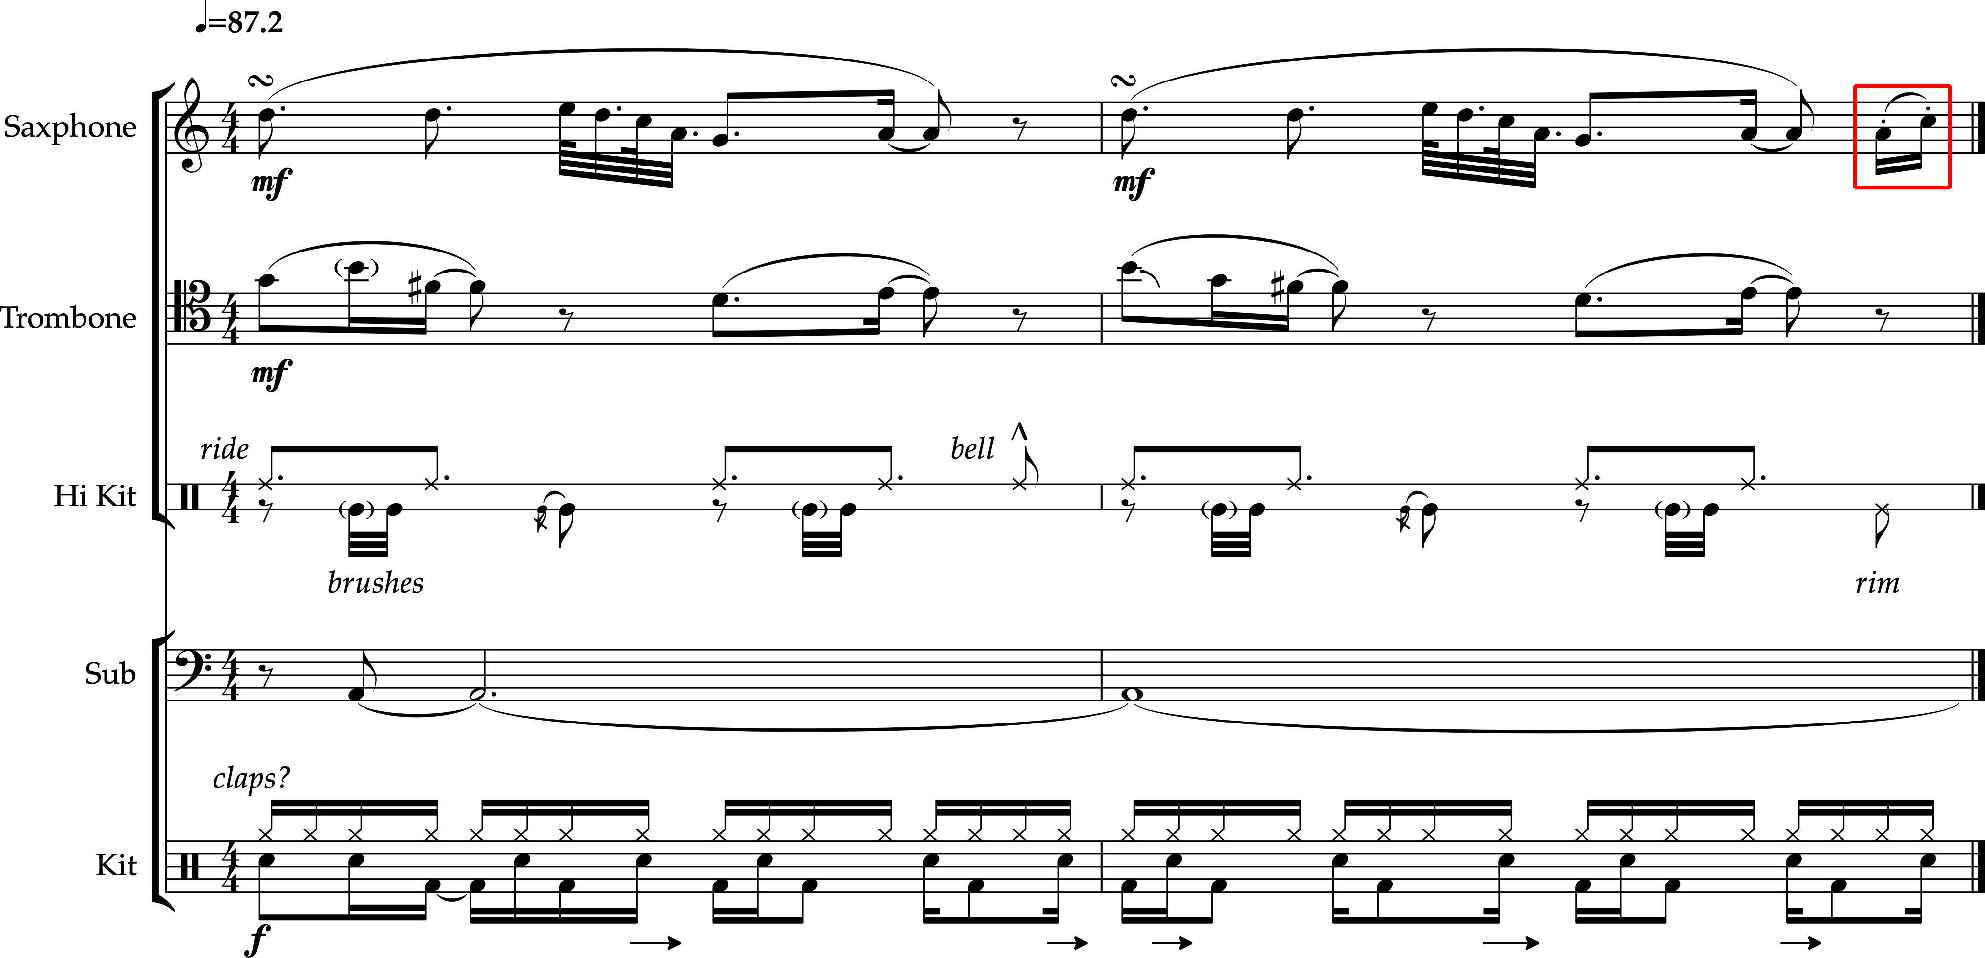
\includegraphics[width=\textwidth]{images/figures/chp 02/043053rigamortusnoslip.pdf}
    \caption{Snapshot of the first verse in ``Rigamortus,'' 0:43-0:55.}
    \label{fig:rigamortusnoslip}
\end{figure}


Although the track's musical components are simplified, Willie B and Sounwave vary their samples and 
loops subtly within the repetitive texture. As Table~\ref{tab:rigamortus} notes, sample choking features
heavily in this track, with the lead sample from ``The Thorn'' rarely playing intact once introduced. 
With Lamar's vocals taking on the ``tendency to fill up sonic space'' of Wilson's heterogeneous
sound-ideal,\footnote{\cite{ollywilsonHeterogeneousSoundIdeal1992}, 328.} the producers opt for 
sample choking as a method of alteration because of its subtractive function, and they employ it 
most drastically when Lamar's vocals reach an apex in Verse 2B. From 2:06-2:18, the lead sample drops
out for measures at a time time, drawing attention to the increasing rhythmic rapidity of Lamar's flow.
Their implementation of sample choking as a tool exists in conversation with Lamar's musical decisions.

\begin{figure}[htp]
    \centering
    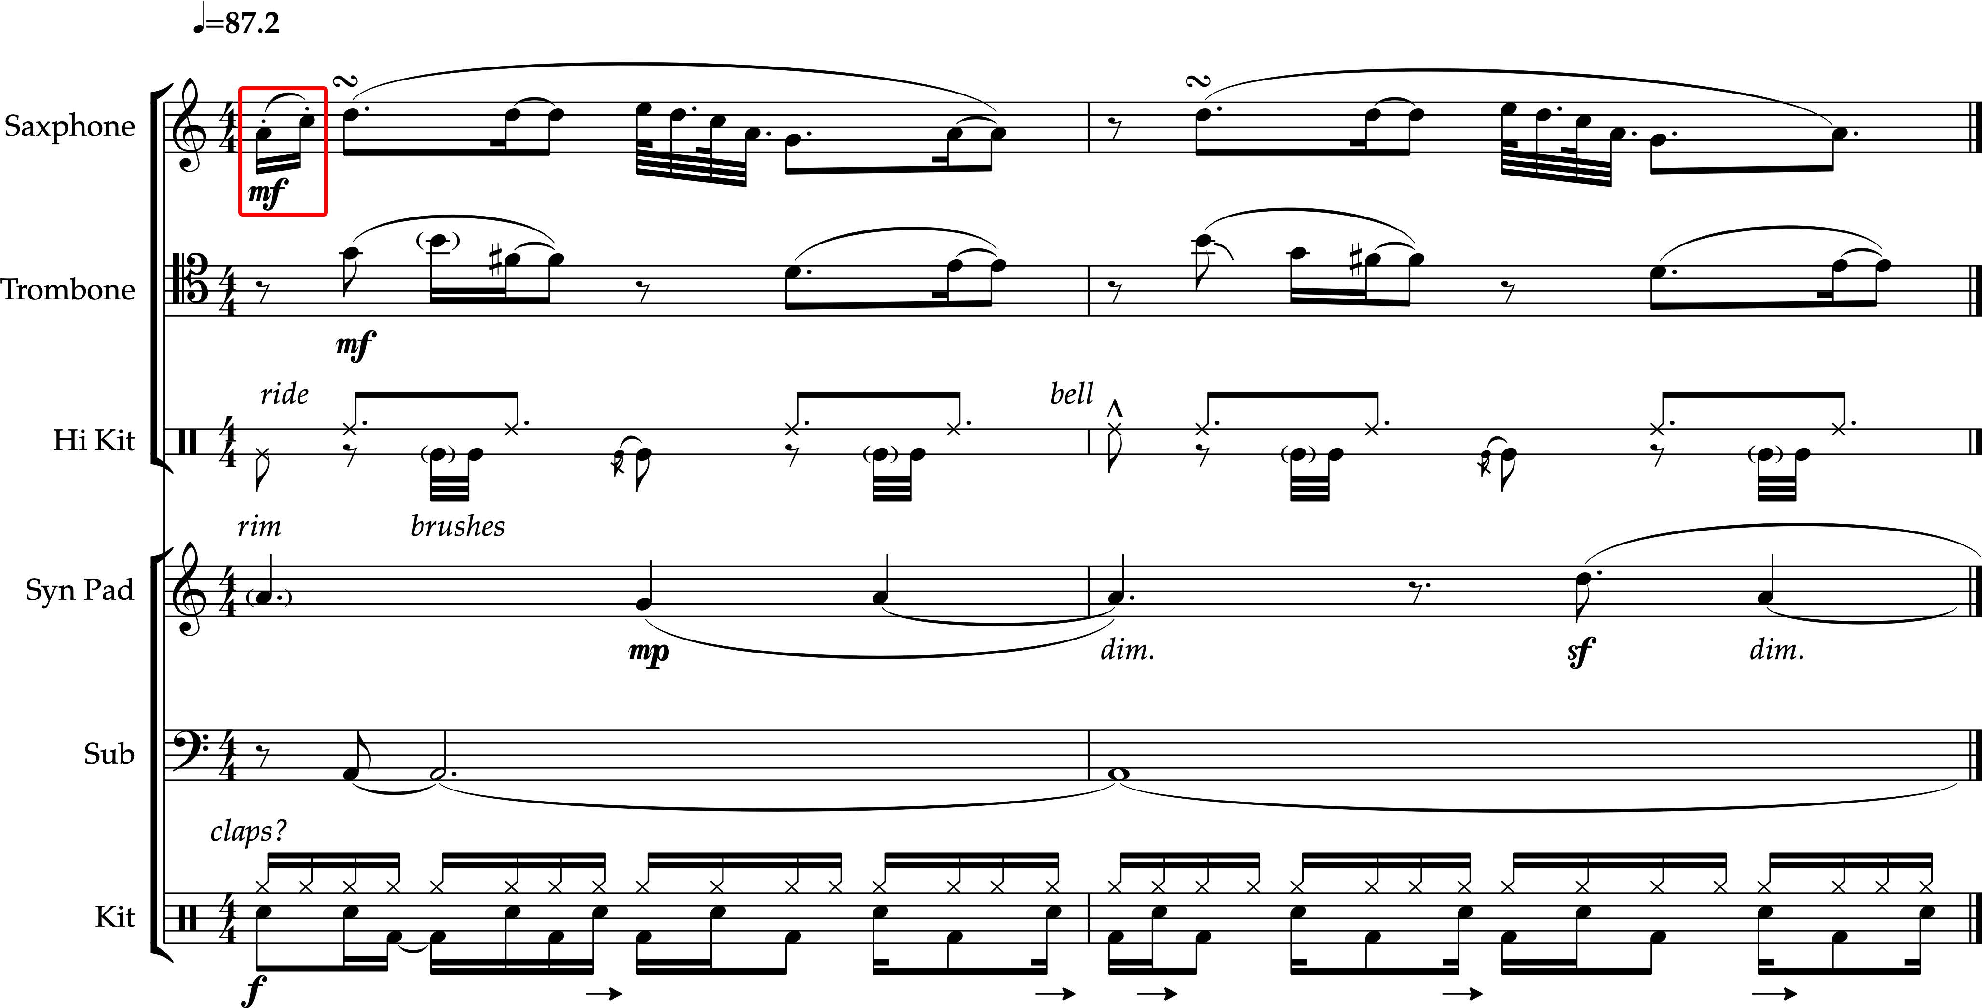
\includegraphics[width=\textwidth]{images/figures/chp 02/126137rigamortusslip.pdf}
    \caption{Snapshot of the first hook in ``Rigamortus,'' 1:26-1:37.}
    \label{fig:rigamortusslip}
\end{figure}

Even more subtly, the producers employ sample slippage as a method of altering the beat in ``Rigamortus.''
Due to the expressive and delayed re-triggering of the lead sample, the microrhythmic relationship 
between musical elements from ``The Thorn'' and the producers' additions exist throughout the work 
in a state of rhythmic flux.\footnote{The phenomenon of sample slippage dovetails with Anne Danielsen's 
work on the Beat Bin and rhythmic tolerance (see \cite{annedanielsenHereThereEverywhere2016}, 
29\textit{ff}. The affective result of these shifts creates a listening experience akin to phasing, 
as samples (albeit sonically discrete ones) move in and out of sync with each other.} Where the pickup
gesture in the saxophone (boxed in red in Figures~\ref{fig:thethornfull}~and~\ref{fig:rigamortusnoslip})
demarcated the end of the lead sample when it was first heard, the sample shifts backwards in the musical
texture throughout the first verse. By the hook, the sample is displaced from its original position in 
the groove, and, as Figure~\ref{fig:rigamortusslip} shows, the pickup figure sounds as a downbeat rather
than a pickup. Both the drum sequence and Lamar's call-and-response vocal articulate this downbeat, which
the saxophone, trombone and sub-bass enter behind by two sixteenth notes. The producers' use of slippage,
then, allows for a sample, which is typically sonically fixed, to become rhythmically fluid.

Willie B and Sounwave's production on ``Rigamortus'' challenges a listener's sense that the lead 
sample on the track is uniformly repetitive. While choking and slipping serve as their primary methods
of altering the sample itself, they also create variety in the beat through the use of digitally-recorded
loops, layering in and out of the mix throughout the track. These loops are all used in conversation 
with Lamar's vocal delivery, helping to create an even greater sense of variety within the musical 
texture. Compared to Madlib's approach to beatmaking, which created variety primarily through the
juxtaposition of disparate samples, Willie B and Sounwave track new elements around the lead sample, 
widening the sample's context. This links the practice of creating variety in sample-based hip-hop 
to another style of production: live-tracked recording.

%\clearpage
\section{Live-Tracked Case Studies}
The second half of this chapter shifts in focus from beats that are sample-based to beats that are
live-tracked. While the distinction between these approaches remains helpful to identifying and describing
the components of a musical texture, it is not a distinction that holds significance beyond this. 
Schloss's ethnographic work in the early-to-mid 2000s Seattle hip-hop scene leads him to the conclusion
that ``the distinction between sample-based and non-sample-based hip-hop is a distinction in
genre.''\footnote{\cite{josephgschlossMakingBeatsArt2004}, 5.} I do not intend to bring in 
such a distinction.

While Schloss's framework may help to explain works in early 2000s underground hip-hop, it becomes
increasingly problematic within modern approaches to music making. When a beat is created in a DAW, 
the distinction between sampling vinyl, using pre-recorded audio or MIDI loops, and live-tracking an
instrument becomes less drastic than within older recording hardware. With the following examples, I aim
to demonstrate that beats are not underground because of the means of generating musical material, but 
rather because of the manipulation of material thereafter.

\phantomsection
\subsection*{\centering Milo's ``Rabblerouse''}
\addcontentsline{toc}{subsection}{Milo's ``Rabblerouse''}

\begin{table}[ht]
    \centering
        \begin{tabular}{|c|c|c|c|l|}
             \hline
            Section & Timecode & Duration & Sample                  & Note \\ \hline
            Intro   & 0:00     & 4 Bars   &                         & Rhodes extends over boundary \\ \hline
            Verse   & 0:08     & 24 Bars  &                         & \\ \hline
                    & 0:14     &          &                         & Drum glitch \\ \hline
                    & 0:36     &          &                         & Drum glitch, bass recomp. \\ \hline
            Outro   & 0:56     & 4 Bars   &                         & Glich, recomp., and choking \\ \hline
                    & 1:03     &          & \textit{Soul Caliber} 2 & \\ \hline
        \end{tabular}
    \caption{Condensed roadmap to Milo and Kenny Segal's ``Rabblerouse''}
    \label{tab:rabblerouse}
\end{table}

Kenny Segal's instrumental for ``Rabblerouse'' creates variety in a complementary fashion to the 
delivery of Milo's text. As shown in Table~\ref{tab:rabblerouse}, ``Rabblerouse'' consists of a single
twenty-four-bar verse framed by two short musical sequences. The track does not end with music; rather, 
it features an unaccompanied vocal sample of the video game character Yoshimitsu from \emph{Soul Caliber 2},
saying ``overconfidence is the greatest enemy'' before giving a battle cry. The sample links ``Rabblerouse''
as an introductory song fragment to Milo's full LP, \emph{So The Flies Don't Come}. It both propels the
listener into the downbeat of the second track, ``Souvenir,'' and links thematically to a line Milo 
delivers in the penultimate track, ``Napping Under the Echo Tree,'' where Milo names himself as the
``Yoshimitsu of Boyle Heights.'' With both sample selection and music, Segal uses ``Rabblerouse'' to 
create instability, urging the listener on toward the album as a whole.

Several structural levels contribute to the fragmentary nature of this opening track. The track is 
structured around an unconventional six-bar chord loop, played in staccato quarter notes on a Fender
Rhodes. Although functional in an E Dorian modal collection, the expansional loop sounds
unresolved.\footnote{\cite{kyleadamsHarmonicSyntacticMotivic2020}. Adams does not make it a 
requisite condition of the expansional harmonic category to function as a complete phrase, although 
he notes that it commonly will.} The C\#$^{sus4}$ harmony that ends the loop, rather than resolving 
the suspension down, cycles back up to an similarly voiced E$^{sus4}$. The stability of this chord 
loop is also challenged by Milo's vocal entrance, which comes after a conventional four bars. The 
Rhodes progression extends over this formal boundary, offsetting the downbeats being projected by 
rapper and producer.

    \begin{figure}[ht]
        \centering
        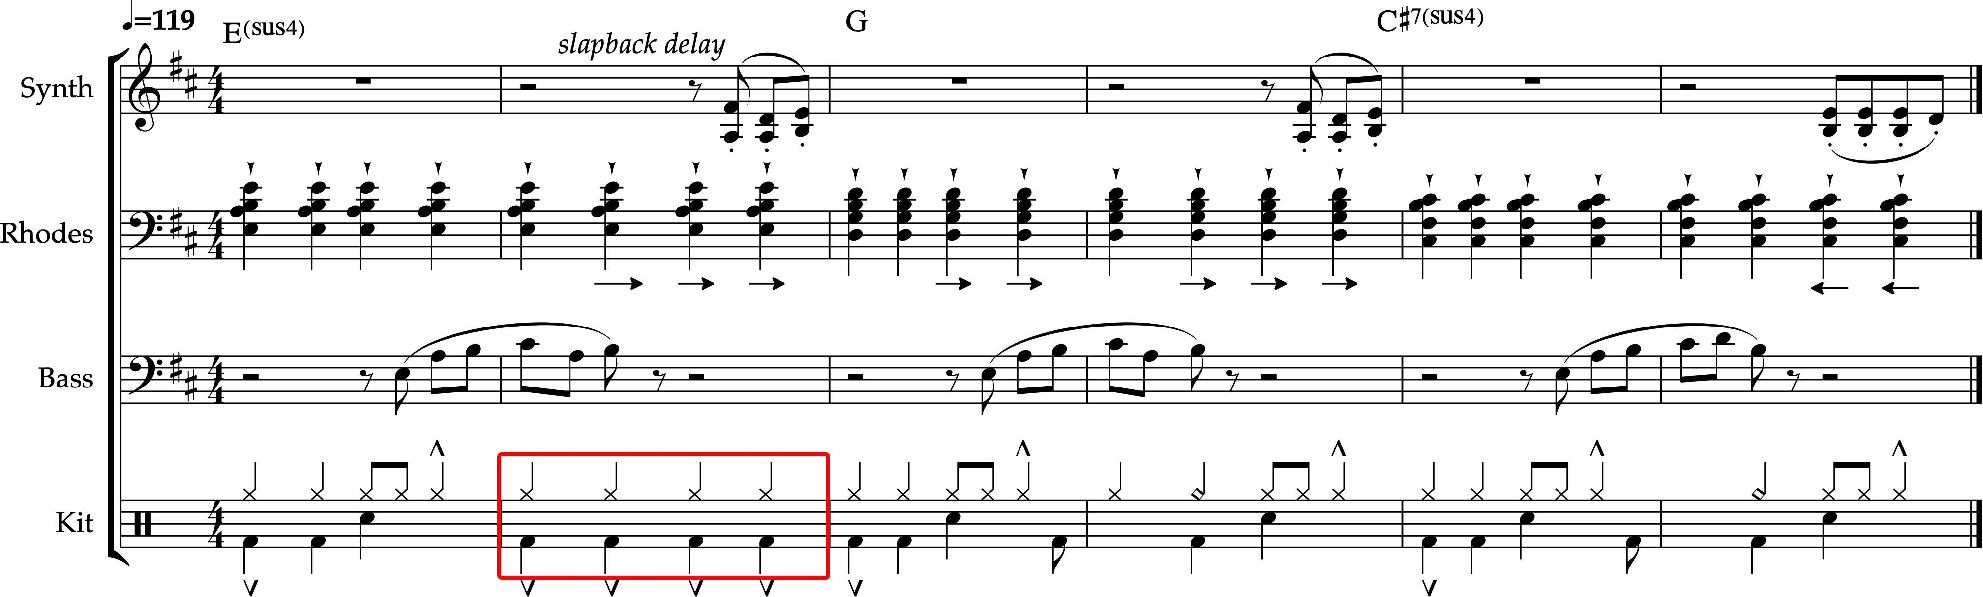
\includegraphics[width=\textwidth]{images/figures/chp 02/012023rabblefirstglitch.pdf}
        \caption{Snapshot of the first drum glitch in ``Rabblerouse,'' 0:12-0:23.}
        \label{fig:rabblefirstglitch}
    \end{figure}

Segal's first notable use of a method of alteration occurs as a response to this dissonance between
the agogic stress of the rapped text and the beat. Boxed in red in Figure~\ref{fig:rabblefirstglitch}, 
Segal uses a glitch in the drum loop to articulate a new point of agogic stress. Measure 2 of the 
figure shows a repetition of four quarter-note kick and hi-hat hits, where Segal has likely selected 
a portion of the drum loop in his DAW and duplicated it four times, restarting the loop in m. 3. This
instance underscores the textual beginning of a new idea: Milo begins ``The wordsmith gets knee-deeper,
beleaguered'' and Segal's glitch transforms the start of the phrase into an upbeat, so that ``deeper''
becomes the strongest metric point of the phrase. Segal's alteration functions as a partial corrective, 
in response to the overall rhythmic complexity introduced in the play between text and music.

    \begin{figure}[ht]
        \centering
        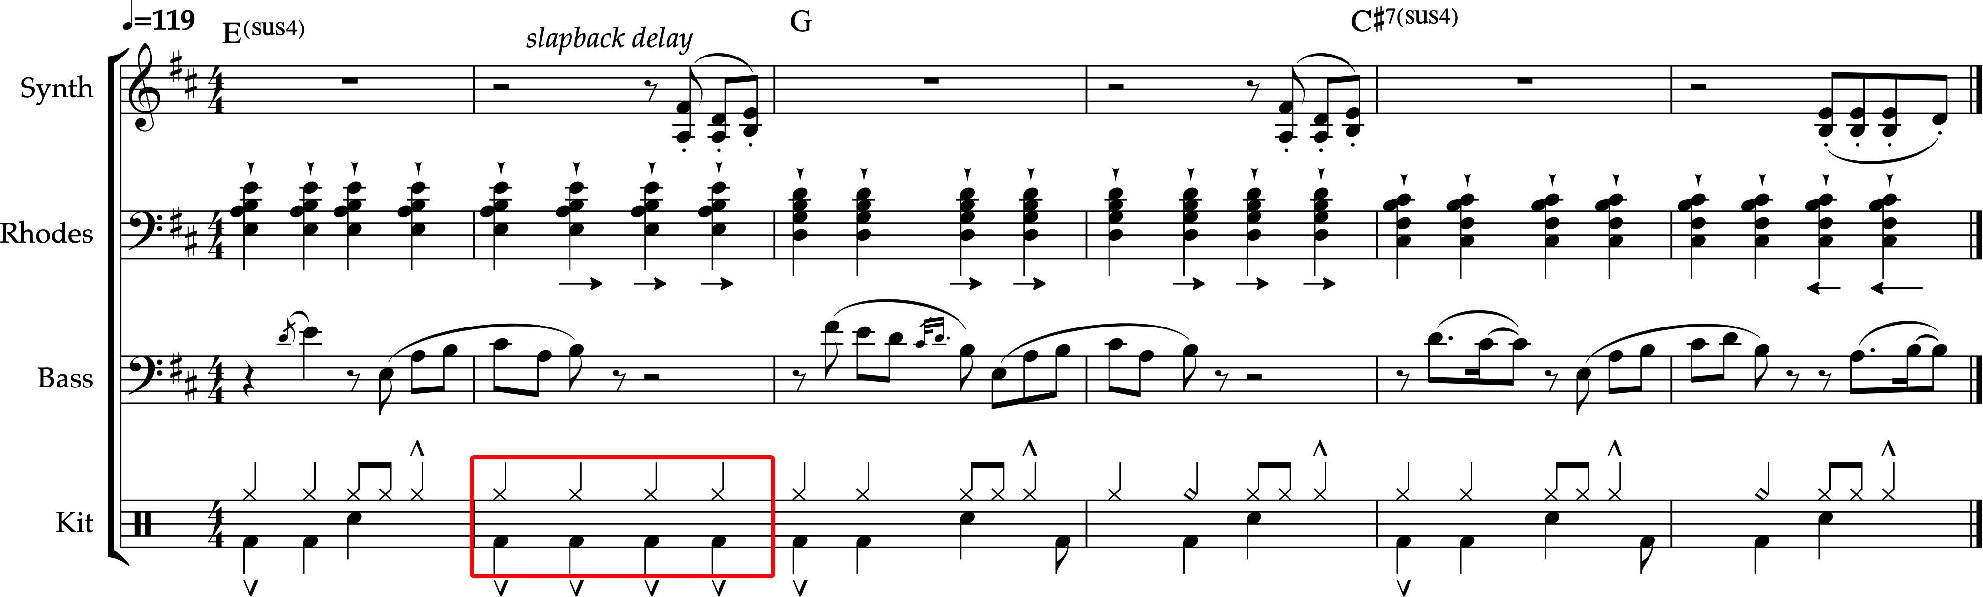
\includegraphics[width=\textwidth]{images/figures/chp 02/036048rabblesecondglitch.pdf}
        \caption{Snapshot of the second drum glitch in ``Rabblerouse,'' 0:36-0:48.}
        \label{fig:rabblesecondglitch}
    \end{figure}

A parallel instance to the first glitch occurs from 0:36-0:48, but its onset is further complicated
by Segal's use of a bass recomposition. Figure~\ref{fig:rabblesecondglitch} shows the loops in this 
moment, with the changes to the bassline implemented by bassist and frequent collaborator of Segal's, 
Mike Parvizi. Parvizi decorates the originally sparse bass lines that begin mid-measure with sleek,
syncopated melodic lead-ins. This busies the texture, while Segal uses another glitch to create agogic 
stress in mm. 2-3. Milo's text \textemdash  ``suits of armor for suicide note authors'' \textemdash again
becomes a point of metric stress, but around this measure, Parvizi's basslines increase the number of
rhythmic onsets within the measure, thereby increasing 
heterogeneity.\footnote{\cite{ollywilsonHeterogeneousSoundIdeal1992}, 328. The ``tendency to create 
rhythmic musical events clash or disagreements of accents'' is the element of the heterogeneous sound 
ideal to which this instance appeals.}

Glitch also functions as the means of suspending rhythmic and metrical clash at the piece's end. As Milo
comes to the end of his verse, Segal uses the same downbeat-repeating drum glitch, pairing it with a 
glitch that extends the E$^{sus4}$ harmony. This point of stasis, though harmonically unresolved, allows
for the listener to hear rhythmic unification for a brief instant, before the texture dissolves and the
Yoshimitsu sample is triggered. Drawing on several methods of altering loops in the beat, Segal brings
together the many fragmentary, disparate pieces of the loop for a brief moment to set a listener up for
what's to come on the record overall.

Segal's fragmentary aesthetic on ``Rabblerouse'' sounds as a mode of alterity because it is uncommon for
a hip-hop beat not to function as a closed loop. The metric dissonance projected from the beginning does
not resolve by the track's end, necessarily drawing a listener in to the text function and pointing 
towards the remaining tracks on the album. This beat is unstable alone, but functions cohesively with 
the sonic palette of Milo's LP \textit{So The Flies Don't Come} as a whole. This technique is predicated 
upon an interest in lyricism and album cohesivity propagated within the underground hip-hop scene.

\phantomsection
\subsection*{\centering billy woods' ``Checkpoints''}
\addcontentsline{toc}{subsection}{billy woods' ``Checkpoints''}

\begin{table}[ht]
    \centering
    \begin{tabular}{|c|c|c|l|}
        \hline
         Section      & Timecode & Duration & Note                          \\ \hline
         Intro        & 0:00     & 8 Bars   & Guitar anacrusis choked       \\ \hline
         Verse 1A     & 0:26     & 22 Bars  & Vocal, synth  anacrusis       \\ \hline
                      & 0:40     &          & Guitar, synth recomp          \\ \hline
         Verse 1B     & 1:06     &          & Synth, drum recomp            \\ \hline
         Interlude 1  & 1:40     & 4 Bars   &                               \\ \hline
         Hook?        & 1:51     & 4 Bars   & All parts anacrusis           \\ \hline
         Interlude 2  & 2:06     & 4 Bars   &                               \\ \hline
         Verse 2      & 2:20     & 15 Bars  & Synth anacrusis glitch        \\ \hline
         
    \end{tabular}
    \caption{Condensed roadmap to billy woods and Kenny Segal's ``Checkpoints.''}
    \label{tab:checkpoints}
\end{table}

Segal also served as the beatmaker for billy woods' ``Checkpoints'' and the \textit{Hiding Places} LP 
from which it comes. Comparing his production techniques across projects for two different emcees shows 
how Segal uses them in response both the artist and the work itself, articulating identity uniquely for 
each. Compared to ``Rabblerouse'' with Milo, Segal's instrumentation on ``Checkpoints'' is at once sparser
and more timbrally intense; the choice to use low register electric guitar with a throatier sound matches 
the more aggressive vocal style woods' employs throughout the track. Similarly to ``Rabblerouse,'' Segal
seems to respond to the text in his articulation of form, working with woods to use techniques that help
create formal contrast. Table~\ref{tab:checkpoints} shows the main formal features: a brief introduction,
followed by two verses of varied lengths, which are divided by an interlude and short vocal section that
could potentially function as the song's hook.

A significant element of the beat is its use of anticipation and anacrusis throughout the 
track.\footnote{I use the term anacrusis as opposed to pickup here because the track does not contain
the final two beats. In the fifteenth bar of the second verse, woods raps through beat two, before 
a static signal sounds for a beat, cutting off before beat four.} Following woods' entrances which 
nearly always come two bars before a downbeat, Segal uses the space beneath that to introduce every 
texture before the downbeat where a loop might be expected to start. Figure~\ref{fig:checkpointsintro} 
shows the entrance of each element from 0:26-0:39 when woods' first verse enters. Accompanying his 
two-beat anacrusis, Segal employs a high synth leadline paired with the guitar loop outlining an F-sharp
power chord. An eighth note before the downbeat, the guitar oscillates to a G harmony, supported by an
anticipation in the kick drum. These anticipations create some rhythmic disorientation in contrast 
to the snare drum, which very clearly articulates backbeats in the section.

    \begin{figure}[ht]
        \centering
        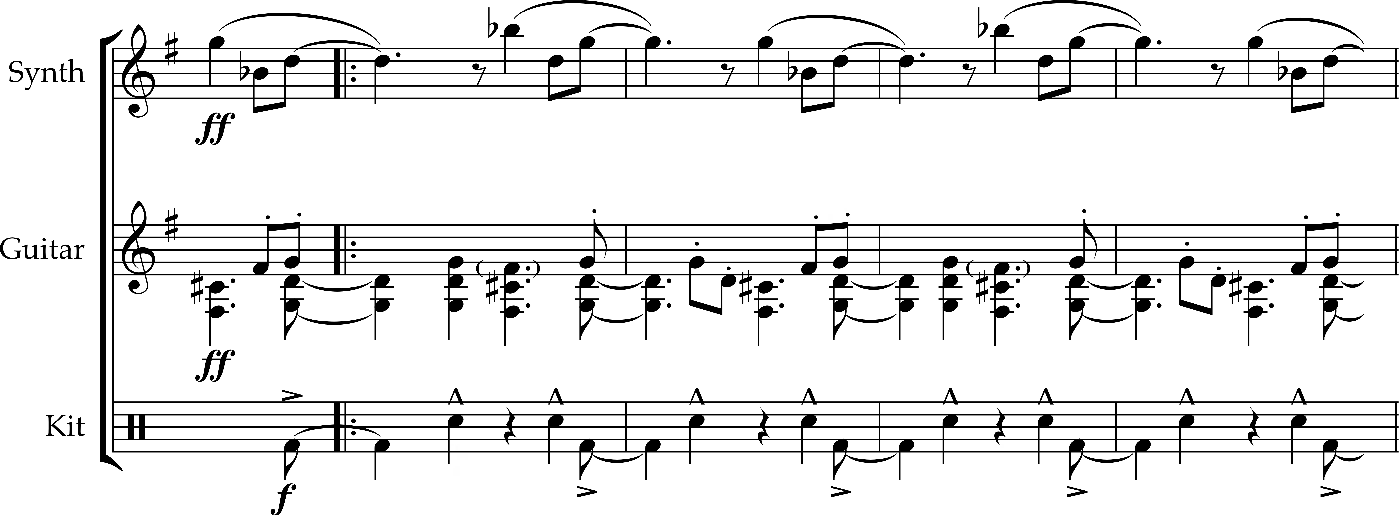
\includegraphics[width=\textwidth]{images/figures/chp 02/026039checkpointsintro.pdf}
        \caption{Snapshot of the beginning of the first verse of ``Checkpoints,'' 0:26-0:39.}
        \label{fig:checkpointsintro}
    \end{figure}

Segal introduces variety into the texture using two significant recompositions of musical material. 
Shown in Figure~\ref{fig:checkpointsmain}, Segal uses a drum recomposition to divide the first verse 
into two eleven-bar units. Following the structure outlined by the kick-snare pattern up to this point,
a crash cymbal emphasizes the downbeat anticipation in the kick, and the same sample sounds a step 
higher along with an open hi-hat sample to emphasize the snare's backbeats. This rock-like groove 
serves as Segal's means of creating variation at an unexpected point of formal division.

    \begin{figure}[ht]
        \centering
        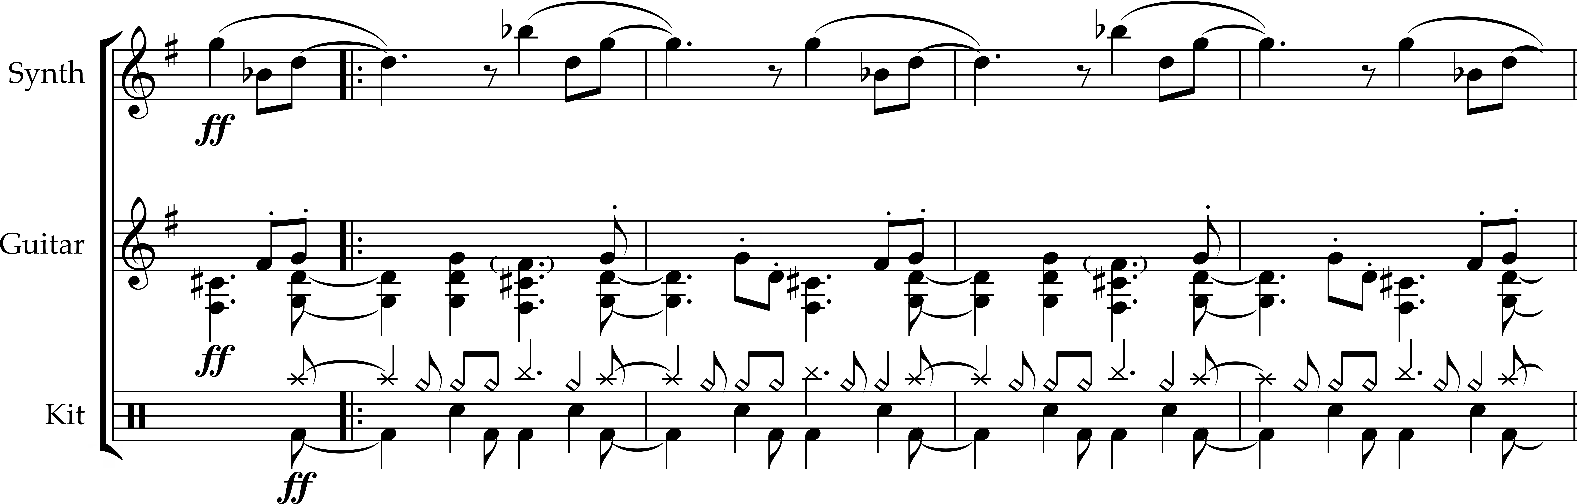
\includegraphics[width=\textwidth]{images/figures/chp 02/106119checkpointsmain.pdf}
        \caption{Snapshot of the drum recomposition in ``Checkpoints,'' 1:06:-1:19.}
        \label{fig:checkpointsmain}
    \end{figure}

Even with woods' vocal delivery signalling a change, the drum recomposition can catch the listener
off-guard. New additions to the drum sequence disrupt the sense of regularity established by the 
kick-snare alternation, especially at a point of division eleven bars into a verse. Moreover, Segal's
choice of drum timbres challenge a listener's sense of genre. Throughout \emph{Hiding Places}, Segal
intentionally uses ``distorted guitars and psych-rock timbres,'' playing with stylistic allusion on 
tracks like ``Checkpoints,'' ``Spongebob,'' and ``Speak Gently.''\footnote{Quoted in 
\cite{backwoodzhiphopKennySegalPresents2019}.} On ``Checkpoints'' specifically, the full drum pattern
engages in allusion while introducing variety.

    \begin{figure}[ht]
        \centering
        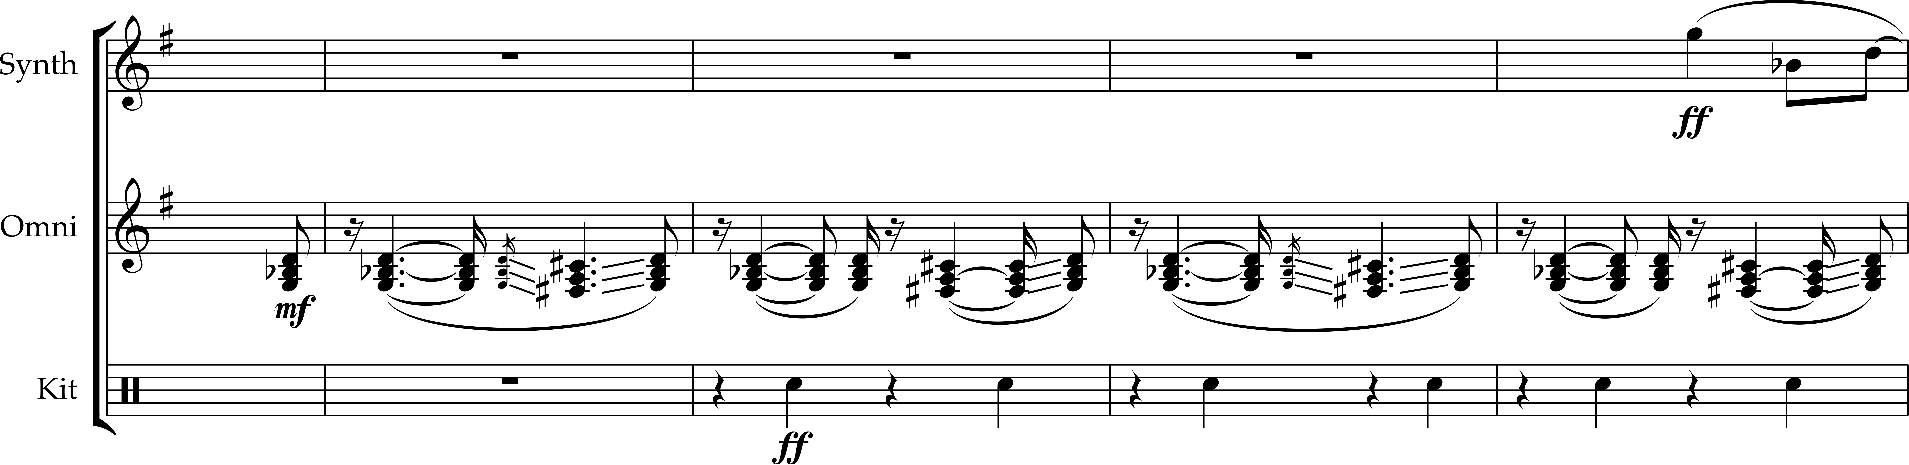
\includegraphics[width=\textwidth]{images/figures/chp 02/040053checkpointsrecomp.pdf}
        \caption{Snapshot of the chordal recomposition in ``Checkpoints,'' 0:40-0:53.}
        \label{fig:checkpointsrecomp}
    \end{figure}

Segal uses recomposition to create formal and textural variety with another significant musical 
element: the chord progression. Figure~\ref{fig:checkpointsrecomp} shows its first entrance, midway 
through Verse 1A. Still in rhythmic anticipation of the downbeat, the chordal loop switches from a 
guitar outlining G and F-sharp power chords to a Suzuki Omnichord planing between G-minor and F-sharp
major triads in the same low-mid layer. Although this recomposition switches instruments, the paired 
range and similar rhythmic placement of the chordal loops aligns the function of these two parts, 
introducing contrasting timbres that take on the same function within the overall 
texture.\footnote{This use of timbral shifts within a shared musical range creates an unblended,
heterogeneous quality within the chordal accompaniment, in keeping with Wilson's heterogeneous 
sound ideal (\textit{cf}.  \cite{ollywilsonHeterogeneousSoundIdeal1992}, 329).}

Each time the chordal recomposition enters, Segal removes all other accompanimental layers
before reintroducing the snare and synth lead. This thinned out texture takes on two distinct 
formal roles. Within the first verse, Segal uses this recomposition to reduce the energy of the 
beat, making the drum recomposition even more drastic when it re-enters with the guitar twenty 
seconds later. This first instance of recomposition allows for a change in energy, creating an 
internal division of the first two verse-parts.

At 1:40, Segal brings the chordal recomposition back to signal a boundary between the verse and 
what follows. For four bars after Verse 1B, the Omnichord and snare sound together, before woods 
re-enters with new text, underscored by the drum kit kit, synth, and guitar also for four bars. 
Segal then switches back to the Omnichord and snare texture for another four bars in anticipation 
of a more fully-orchestrated Verse 2. In these second and third entrances, the recomposition functions
as a formal interlude, affording a weight to the four bars of music and text between them. Indeed, 
woods' text in this section has a certain thematic weight to it; Segal's delineation of form with
recompostion thus helps draw this out.

Segal's use of timbral contrast and sequencing of recompositions within ``Checkpoints'' create
an internal variety within the song form, and plays with the broader, generic context of underground
hip-hop. In Segal's memory of mainstream rap history, the use of rock-like timbres in hip-hop has, 
on occasion, yielded ``disastrously wack results.''\footnote{\cite{backwoodzhiphopKennySegalPresents2019}.}
His choice to navigate this potentially-treacherous sonic territory reveals his willingness to
re-contextualize musical material in play with normative, mainstream expectations. At the same 
time, the use of timbre in ``Checkpoints'' illustrates a desire to do so with specific aesthetic
and compositional ends in mind. Like the sonic profile of his production on \textit{So the Flies 
Don't Come}, this track (and \textit{Hiding Places} as a whole) seem sonically linked to the text, 
themes, and vocal style of the emcee the track exists in service to. Segal's primary concern as a 
producer, then, seems to be sounding an identity \emph{with} the emcee.

%\clearpage
\section{The Co-Creation of Underground Identity}
This chapter positions underground hip-hop producers as coauthors in the creation of a underground
identity with the emcee. Because their work is largely non-textual, underground producers use
normative expectations for form and content in a hip-hop track as a basis for a type of sonic play
that manifests as heterogeneity within a hip-hop beat's construction. Underground producers create
forms that are non-normative, articulating them through sample and loop juxtapositions, and ascribing
formal rhetoric to different portions of the beat through their choice of sequencing. Within 
instrumental sections, producers create heterogeneity with a variety of techniques for manipulating 
sound, four of which I have explored in depth during this chapter. Formal and compositional variety 
functions as a sonic metaphor for the non-normativity of the emcees who rap over these tracks.